% Options for packages loaded elsewhere
\PassOptionsToPackage{unicode}{hyperref}
\PassOptionsToPackage{hyphens}{url}
%
\documentclass[
]{article}
\usepackage{lmodern}
\usepackage{amssymb,amsmath}
\usepackage{ifxetex,ifluatex}
\ifnum 0\ifxetex 1\fi\ifluatex 1\fi=0 % if pdftex
  \usepackage[T1]{fontenc}
  \usepackage[utf8]{inputenc}
  \usepackage{textcomp} % provide euro and other symbols
\else % if luatex or xetex
  \usepackage{unicode-math}
  \defaultfontfeatures{Scale=MatchLowercase}
  \defaultfontfeatures[\rmfamily]{Ligatures=TeX,Scale=1}
\fi
% Use upquote if available, for straight quotes in verbatim environments
\IfFileExists{upquote.sty}{\usepackage{upquote}}{}
\IfFileExists{microtype.sty}{% use microtype if available
  \usepackage[]{microtype}
  \UseMicrotypeSet[protrusion]{basicmath} % disable protrusion for tt fonts
}{}
\makeatletter
\@ifundefined{KOMAClassName}{% if non-KOMA class
  \IfFileExists{parskip.sty}{%
    \usepackage{parskip}
  }{% else
    \setlength{\parindent}{0pt}
    \setlength{\parskip}{6pt plus 2pt minus 1pt}}
}{% if KOMA class
  \KOMAoptions{parskip=half}}
\makeatother
\usepackage{xcolor}
\IfFileExists{xurl.sty}{\usepackage{xurl}}{} % add URL line breaks if available
\IfFileExists{bookmark.sty}{\usepackage{bookmark}}{\usepackage{hyperref}}
\hypersetup{
  pdftitle={A6\_Joslin\_Lauryn},
  pdfauthor={Lauryn Joslin},
  hidelinks,
  pdfcreator={LaTeX via pandoc}}
\urlstyle{same} % disable monospaced font for URLs
\usepackage[margin=1in]{geometry}
\usepackage{color}
\usepackage{fancyvrb}
\newcommand{\VerbBar}{|}
\newcommand{\VERB}{\Verb[commandchars=\\\{\}]}
\DefineVerbatimEnvironment{Highlighting}{Verbatim}{commandchars=\\\{\}}
% Add ',fontsize=\small' for more characters per line
\usepackage{framed}
\definecolor{shadecolor}{RGB}{248,248,248}
\newenvironment{Shaded}{\begin{snugshade}}{\end{snugshade}}
\newcommand{\AlertTok}[1]{\textcolor[rgb]{0.94,0.16,0.16}{#1}}
\newcommand{\AnnotationTok}[1]{\textcolor[rgb]{0.56,0.35,0.01}{\textbf{\textit{#1}}}}
\newcommand{\AttributeTok}[1]{\textcolor[rgb]{0.77,0.63,0.00}{#1}}
\newcommand{\BaseNTok}[1]{\textcolor[rgb]{0.00,0.00,0.81}{#1}}
\newcommand{\BuiltInTok}[1]{#1}
\newcommand{\CharTok}[1]{\textcolor[rgb]{0.31,0.60,0.02}{#1}}
\newcommand{\CommentTok}[1]{\textcolor[rgb]{0.56,0.35,0.01}{\textit{#1}}}
\newcommand{\CommentVarTok}[1]{\textcolor[rgb]{0.56,0.35,0.01}{\textbf{\textit{#1}}}}
\newcommand{\ConstantTok}[1]{\textcolor[rgb]{0.00,0.00,0.00}{#1}}
\newcommand{\ControlFlowTok}[1]{\textcolor[rgb]{0.13,0.29,0.53}{\textbf{#1}}}
\newcommand{\DataTypeTok}[1]{\textcolor[rgb]{0.13,0.29,0.53}{#1}}
\newcommand{\DecValTok}[1]{\textcolor[rgb]{0.00,0.00,0.81}{#1}}
\newcommand{\DocumentationTok}[1]{\textcolor[rgb]{0.56,0.35,0.01}{\textbf{\textit{#1}}}}
\newcommand{\ErrorTok}[1]{\textcolor[rgb]{0.64,0.00,0.00}{\textbf{#1}}}
\newcommand{\ExtensionTok}[1]{#1}
\newcommand{\FloatTok}[1]{\textcolor[rgb]{0.00,0.00,0.81}{#1}}
\newcommand{\FunctionTok}[1]{\textcolor[rgb]{0.00,0.00,0.00}{#1}}
\newcommand{\ImportTok}[1]{#1}
\newcommand{\InformationTok}[1]{\textcolor[rgb]{0.56,0.35,0.01}{\textbf{\textit{#1}}}}
\newcommand{\KeywordTok}[1]{\textcolor[rgb]{0.13,0.29,0.53}{\textbf{#1}}}
\newcommand{\NormalTok}[1]{#1}
\newcommand{\OperatorTok}[1]{\textcolor[rgb]{0.81,0.36,0.00}{\textbf{#1}}}
\newcommand{\OtherTok}[1]{\textcolor[rgb]{0.56,0.35,0.01}{#1}}
\newcommand{\PreprocessorTok}[1]{\textcolor[rgb]{0.56,0.35,0.01}{\textit{#1}}}
\newcommand{\RegionMarkerTok}[1]{#1}
\newcommand{\SpecialCharTok}[1]{\textcolor[rgb]{0.00,0.00,0.00}{#1}}
\newcommand{\SpecialStringTok}[1]{\textcolor[rgb]{0.31,0.60,0.02}{#1}}
\newcommand{\StringTok}[1]{\textcolor[rgb]{0.31,0.60,0.02}{#1}}
\newcommand{\VariableTok}[1]{\textcolor[rgb]{0.00,0.00,0.00}{#1}}
\newcommand{\VerbatimStringTok}[1]{\textcolor[rgb]{0.31,0.60,0.02}{#1}}
\newcommand{\WarningTok}[1]{\textcolor[rgb]{0.56,0.35,0.01}{\textbf{\textit{#1}}}}
\usepackage{graphicx,grffile}
\makeatletter
\def\maxwidth{\ifdim\Gin@nat@width>\linewidth\linewidth\else\Gin@nat@width\fi}
\def\maxheight{\ifdim\Gin@nat@height>\textheight\textheight\else\Gin@nat@height\fi}
\makeatother
% Scale images if necessary, so that they will not overflow the page
% margins by default, and it is still possible to overwrite the defaults
% using explicit options in \includegraphics[width, height, ...]{}
\setkeys{Gin}{width=\maxwidth,height=\maxheight,keepaspectratio}
% Set default figure placement to htbp
\makeatletter
\def\fps@figure{htbp}
\makeatother
\setlength{\emergencystretch}{3em} % prevent overfull lines
\providecommand{\tightlist}{%
  \setlength{\itemsep}{0pt}\setlength{\parskip}{0pt}}
\setcounter{secnumdepth}{-\maxdimen} % remove section numbering

\title{A6\_Joslin\_Lauryn}
\author{Lauryn Joslin}
\date{09/03/2022}

\begin{document}
\maketitle

\#Dragon Phylogeny : Assignment 7

\#\#March 9th 2022

Coding the dragons, was manually added to original nexus

\textbf{Dragon 1} , From Disney's Hercules - Menken, Alan. Disney's
Hercules. {[}United States{]} : Milwaukee, WI :Wonderland Music Co.~and
Walt Disney Music Co.~; Distributed by H. Leonard, 1997. :1HerculesX

\begin{figure}
\centering
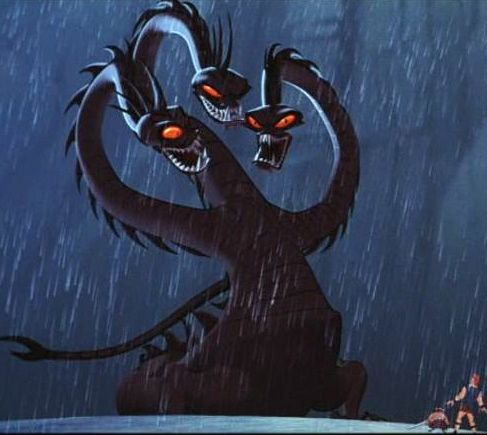
\includegraphics{"/Users/temp/Dropbox/A7_Joslin_Lauryn/images/dragon1.jpeg"}
\caption{dragon 1 1HerculesX}
\end{figure}

1101 1111 01 ???? 011000 000 001 1 110 ? ? ?????? 110000 000001 1000 00
0001 ? ?????? ? ?? 1 00 00 ???

appendages 2 1101 mass \textgreater4x human 1111 body type elongate 01
claw type unknown ???? Dorsal ridges spike 011000 Ear absent 000 eye
large 001 eye position forward 1 horn long 110 nose position ? nose
morhology ? skin dorsal ?????? skin head smooth 110000 skin ventral
plates 000001 snout blunt 1000 tail split 00 teeth fangs + other 0001
toes ? Toe num ?????? tongue length ? tongue morph ?? ventral plates y 1
whiskers 00 wing struct 00 wing type ???

\textbf{Dragon 2} - from BBC Merlin TV series 2008-2012: 2MerlinXXX

\begin{figure}
\centering
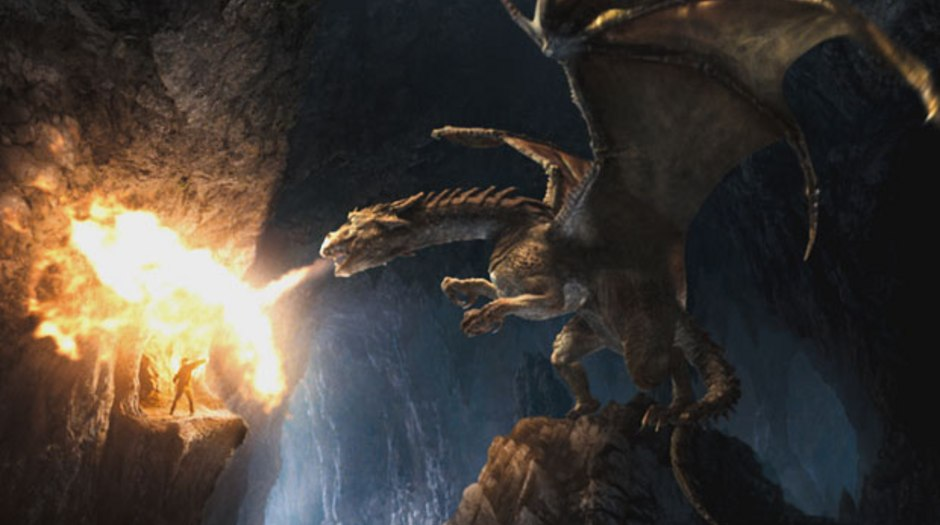
\includegraphics{"/Users/temp/Dropbox/A7_Joslin_Lauryn/images/dragon2.jpeg"}
\caption{dragon 2 2MerlinXXX}
\end{figure}

1001 1111 00 0011 011000 000 100 0 000 1 1 000000 100000 100000 1100 10
1100 0 100000 ? ?? 0 00 11 100

appendages 4 1001 mass \textgreater4x human 1111 body type 00 claw type
0011 Dorsal ridges spike 011000 Ear absent 000 eye large 100 eye
position 0 horn 000 nose position 1 nose morhology 1 skin dorsal 000000
skin head 100000 skin ventral 100000 snout 1100 tail 10 teeth 1100 toes
0 Toe num 100000 tongue length ? tongue morph ?? ventral plates 0
whiskers 00 wing struct 11 wing type 100

\textbf{Dragon 3} - From the cover of the book ``The Dragons of Wayward
Crescent: Gruffen'' by Chris D'Lacy 2009: 3WaywardXX

\begin{figure}
\centering

\includegraphics{"/Users/temp/Dropbox/A7_Joslin_Lauryn/images/dragon3.jpeg"}
\caption{dragon 3 3WaywardXX}
\end{figure}

1001 ???? 00 0010 010000 010 000 0 000 1 1 000000 000000 000001 1110 01
???? 0 111000 ? ?? 1 00 11 100

appendages 4 1001 mass ???? body type 00 claw type 0010 Dorsal ridges
spike 010000 Ear 010 eye 000 eye position 0 horn 000 nose position 1
nose morhology 1 skin dorsal 000000 skin head 000000 skin ventral 000001
snout 1110 tail 01 teeth ???? toes 0 Toe num 111000 tongue length ?
tongue morph ?? ventral plates 1 whiskers 00 wing struct 11 wing type
100

\begin{Shaded}
\begin{Highlighting}[]
\KeywordTok{library}\NormalTok{(ape)}
\KeywordTok{library}\NormalTok{(ggplot2)}
\KeywordTok{library}\NormalTok{(reshape2)}
\KeywordTok{library}\NormalTok{(ggtree)}
\end{Highlighting}
\end{Shaded}

\begin{verbatim}
## ggtree v3.2.1  For help: https://yulab-smu.top/treedata-book/
## 
## If you use ggtree in published research, please cite the most appropriate paper(s):
## 
## 1. Guangchuang Yu. Using ggtree to visualize data on tree-like structures. Current Protocols in Bioinformatics. 2020, 69:e96. doi:10.1002/cpbi.96
## 2. Guangchuang Yu, Tommy Tsan-Yuk Lam, Huachen Zhu, Yi Guan. Two methods for mapping and visualizing associated data on phylogeny using ggtree. Molecular Biology and Evolution. 2018, 35(12):3041-3043. doi:10.1093/molbev/msy194
## 3. Guangchuang Yu, David Smith, Huachen Zhu, Yi Guan, Tommy Tsan-Yuk Lam. ggtree: an R package for visualization and annotation of phylogenetic trees with their covariates and other associated data. Methods in Ecology and Evolution. 2017, 8(1):28-36. doi:10.1111/2041-210X.12628
\end{verbatim}

\begin{verbatim}
## 
## Attaching package: 'ggtree'
\end{verbatim}

\begin{verbatim}
## The following object is masked from 'package:ape':
## 
##     rotate
\end{verbatim}

\begin{Shaded}
\begin{Highlighting}[]
\NormalTok{DragonNex <-}\StringTok{ }\KeywordTok{read.nexus.data}\NormalTok{(}\StringTok{"/Users/temp/Dropbox/A7_Joslin_Lauryn/input/DragonMatrix.nex"}\NormalTok{)}
\end{Highlighting}
\end{Shaded}

\begin{Shaded}
\begin{Highlighting}[]
\NormalTok{Dragondf <-}\StringTok{ }\KeywordTok{data.frame}\NormalTok{(}\KeywordTok{matrix}\NormalTok{(}\KeywordTok{unlist}\NormalTok{(DragonNex), }\DataTypeTok{ncol =} \DecValTok{78}\NormalTok{, }\DataTypeTok{byrow =}\NormalTok{ T))}
\end{Highlighting}
\end{Shaded}

\begin{Shaded}
\begin{Highlighting}[]
\KeywordTok{row.names}\NormalTok{(Dragondf) <-}\StringTok{ }\KeywordTok{names}\NormalTok{(DragonNex)}
\end{Highlighting}
\end{Shaded}

\begin{Shaded}
\begin{Highlighting}[]
\NormalTok{Dragondist <-}\StringTok{ }\KeywordTok{dist}\NormalTok{(Dragondf, }\DataTypeTok{method =} \StringTok{'binary'}\NormalTok{)}
\end{Highlighting}
\end{Shaded}

\begin{verbatim}
## Warning in dist(Dragondf, method = "binary"): NAs introduced by coercion
\end{verbatim}

\begin{Shaded}
\begin{Highlighting}[]
\NormalTok{Dragondistmatrix <-}\StringTok{ }\KeywordTok{as.matrix}\NormalTok{(Dragondist)}
\end{Highlighting}
\end{Shaded}

\begin{Shaded}
\begin{Highlighting}[]
\NormalTok{WeightsDat<-}\KeywordTok{read.csv}\NormalTok{(}\StringTok{"https://colauttilab.github.io/Data/Weights.csv"}\NormalTok{)}
\end{Highlighting}
\end{Shaded}

\begin{Shaded}
\begin{Highlighting}[]
\NormalTok{Weights<-}\KeywordTok{paste0}\NormalTok{(WeightsDat}\OperatorTok{$}\NormalTok{Weight,}\DataTypeTok{collapse=}\StringTok{""}\NormalTok{)}
\NormalTok{Weights<-}\KeywordTok{strsplit}\NormalTok{(Weights,}\DataTypeTok{split=}\StringTok{""}\NormalTok{)[[}\DecValTok{1}\NormalTok{]]}
\end{Highlighting}
\end{Shaded}

\begin{Shaded}
\begin{Highlighting}[]
\NormalTok{WeightsNum<-}\KeywordTok{rep}\NormalTok{(}\OtherTok{NA}\NormalTok{,}\KeywordTok{length}\NormalTok{(Weights))}
\ControlFlowTok{for}\NormalTok{(i }\ControlFlowTok{in} \DecValTok{1}\OperatorTok{:}\KeywordTok{length}\NormalTok{(WeightsNum))\{}
  \ControlFlowTok{if}\NormalTok{(Weights[i] }\OperatorTok\StringTok{ }\NormalTok{LETTERS)\{}
\NormalTok{    WeightsNum[i]<-}\KeywordTok{which}\NormalTok{(LETTERS}\OperatorTok{==}\NormalTok{Weights[i])}\OperatorTok{+}\DecValTok{9}
\NormalTok{  \} }\ControlFlowTok{else}\NormalTok{ \{}
\NormalTok{    WeightsNum[i]<-Weights[i]}
\NormalTok{  \}}
\NormalTok{\}}
\NormalTok{WeightsNum<-}\KeywordTok{as.numeric}\NormalTok{(WeightsNum)}
\end{Highlighting}
\end{Shaded}

\begin{Shaded}
\begin{Highlighting}[]
\NormalTok{WtDragonNex<-DragonNex }
\ControlFlowTok{for}\NormalTok{ (i }\ControlFlowTok{in} \DecValTok{1}\OperatorTok{:}\KeywordTok{length}\NormalTok{(DragonNex))\{}
\NormalTok{  RepWeight<-DragonNex[[i]]}\OperatorTok{==}\DecValTok{1}
\NormalTok{  WtDragonNex[[i]][RepWeight]<-WeightsNum[RepWeight]}
\NormalTok{  RepWeight<-}\OtherTok{NA}
\NormalTok{\}}
\end{Highlighting}
\end{Shaded}

\begin{Shaded}
\begin{Highlighting}[]
\NormalTok{WtDragonNexDF<-}\KeywordTok{data.frame}\NormalTok{(}\KeywordTok{matrix}\NormalTok{(}\KeywordTok{unlist}\NormalTok{(WtDragonNex),}\DataTypeTok{ncol=}\DecValTok{78}\NormalTok{,}\DataTypeTok{byrow=}\NormalTok{T))}
\KeywordTok{row.names}\NormalTok{(WtDragonNexDF)<-}\KeywordTok{names}\NormalTok{(WtDragonNex)}
\NormalTok{WtDragonDist<-}\KeywordTok{dist}\NormalTok{(WtDragonNexDF,}\DataTypeTok{method=}\StringTok{'euclidean'}\NormalTok{)}
\end{Highlighting}
\end{Shaded}

\begin{verbatim}
## Warning in dist(WtDragonNexDF, method = "euclidean"): NAs introduced by coercion
\end{verbatim}

\begin{Shaded}
\begin{Highlighting}[]
\NormalTok{WtDragonDistMat<-}\KeywordTok{as.matrix}\NormalTok{(WtDragonDist)}
\end{Highlighting}
\end{Shaded}

\hypertarget{dragon-phylogeny}{%
\subsection{Dragon Phylogeny}\label{dragon-phylogeny}}

Updated with the 3 new dragons I added, coloured red

\begin{Shaded}
\begin{Highlighting}[]
\NormalTok{WtDragonTree<-}\KeywordTok{fastme.bal}\NormalTok{(WtDragonDist)}
\NormalTok{new<-}\KeywordTok{groupClade}\NormalTok{(WtDragonTree,}\DataTypeTok{.node=}\KeywordTok{c}\NormalTok{(}\DecValTok{96}\NormalTok{))}
\KeywordTok{ggtree}\NormalTok{(new, }\DataTypeTok{layout =} \StringTok{"circular"}\NormalTok{, }\KeywordTok{aes}\NormalTok{(}\DataTypeTok{colour =}\NormalTok{ group), }\DataTypeTok{ignore.negative.edge =} \OtherTok{TRUE}\NormalTok{) }\OperatorTok{+}
\StringTok{  }\KeywordTok{geom_tiplab}\NormalTok{(}\KeywordTok{aes}\NormalTok{(}\DataTypeTok{angle=}\NormalTok{angle),  }\DataTypeTok{size =}\DecValTok{2}\NormalTok{)}\OperatorTok{+}
\StringTok{  }\KeywordTok{scale_color_manual}\NormalTok{(}\DataTypeTok{labels =} \KeywordTok{c}\NormalTok{(}\StringTok{"original"}\NormalTok{, }\StringTok{"new"}\NormalTok{), }\DataTypeTok{values =} \KeywordTok{c}\NormalTok{(}\StringTok{"#000000"}\NormalTok{,}\StringTok{"#e85d04"}\NormalTok{))}\OperatorTok{+}
\KeywordTok{geom_cladelabel}\NormalTok{(}\DataTypeTok{node=}\DecValTok{96}\NormalTok{,}\DataTypeTok{label=}\StringTok{"My New Additions"}\NormalTok{, }\DataTypeTok{offset =} \DecValTok{30}\NormalTok{,}\DataTypeTok{vjust =} \FloatTok{-0.5}\NormalTok{, }\DataTypeTok{hjust=}\FloatTok{0.5}\NormalTok{,}\DataTypeTok{offset.text=}\DecValTok{4}\NormalTok{,}\DataTypeTok{fontsize=}\DecValTok{5}\NormalTok{,}\DataTypeTok{angle=}\DecValTok{96}\NormalTok{, )}\OperatorTok{+}
\StringTok{   }\KeywordTok{labs}\NormalTok{(}\DataTypeTok{colour =} \StringTok{" "}\NormalTok{)}
\end{Highlighting}
\end{Shaded}

\begin{verbatim}
## Warning: The tree contained negative edge length. If you want to ignore the edge, you
## can set 'options(ignore.negative.edge=TRUE)', then re-run ggtree.
\end{verbatim}

\begin{verbatim}
## Warning: Ignoring unknown parameters: ignore.negative.edge
## Ignoring unknown parameters: ignore.negative.edge
\end{verbatim}

\begin{verbatim}
## Warning: Ignoring unknown parameters: vjust
\end{verbatim}

\includegraphics{A7_Joslin_Lauryn_files/figure-latex/unnamed-chunk-13-1.pdf}

\end{document}
